\section{Datacenter Reference Design}

NVIDIA's strategy to accelerate ecosystem readiness is by sharing facility-level reference designs that showcase the feasibility of advanced power architectures. These designs are not rigid specifications, but rather illustrative examples to guide ecosystem partners in aligning on scalable, interoperable solutions for AI Factories. They help identify development opportunities and enable faster co-development of supporting technologies. The reference design will evolve in parallel with NVIDIA's compute product specifications to ensure continued alignment and applicability.

\begin{figure}[h]
\centering
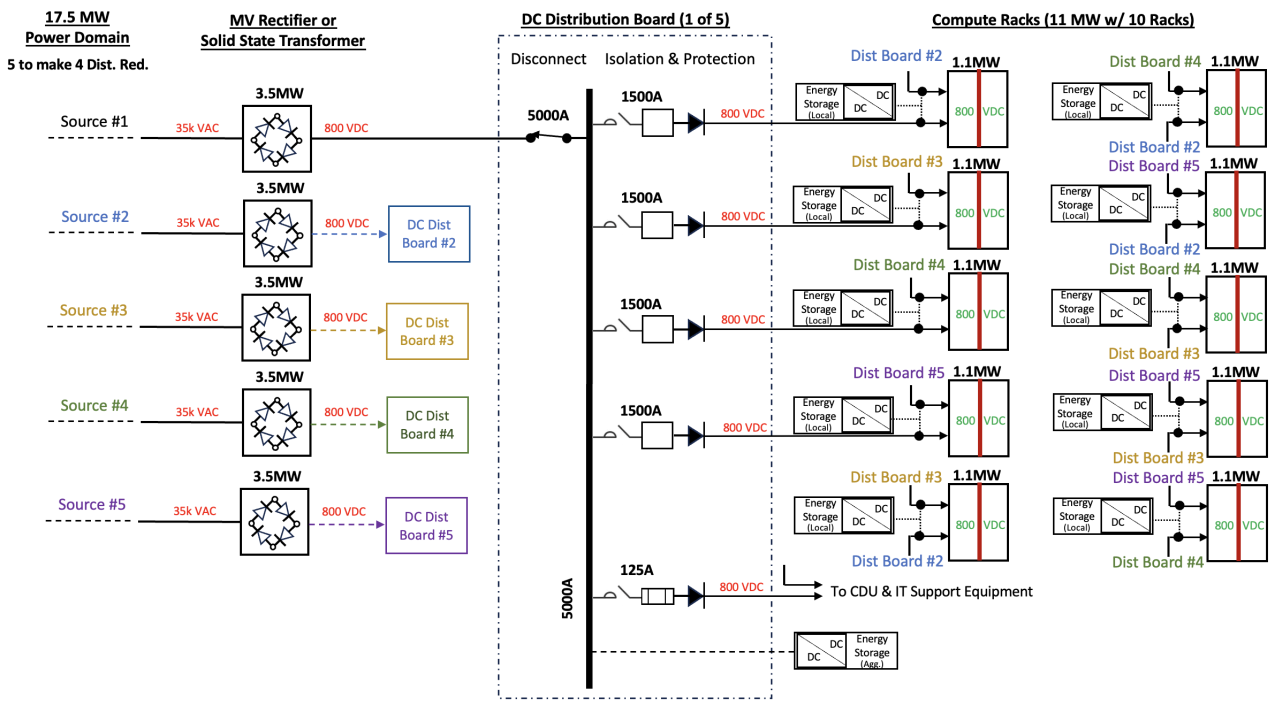
\includegraphics[width=0.8\textwidth]{figures/figure_p16_i1.png}
\caption{800 VDC 17.5 MW Power Block Illustration}
\label{fig:power-block}
\end{figure}

As shown in Figure~\ref{fig:power-block}, the proposed conceptual electrical architecture supports scalable and resilient AI Factory deployment through a 17.5 MW power block leveraging five 3.5 MW medium-voltage (MV) rectifiers in a ``5-to-make-4'' redundant configuration. Each rectifier converts 35 kVAC to 800 VDC and feeds a centralized 5000 A DC distribution board.

Power is distributed via 1500 A busducts or liquid-cooled cables, each equipped with a load-break contactor, solid-state circuit breaker, and blocking diode to ensure safe isolation, fault protection, and containment of fault currents. The system delivers power to four 1.1 MW compute racks along with associated CDUs and IT support equipment.

Each compute rack is supported by local or aggregated energy storage to provide slew-rate control, power smoothing, voltage regulation, and optional backup capability. To maintain concurrent serviceability and uptime, racks are configured with 1+1 redundant feeds sourced from independent rectifiers.

In the event of a single rectifier failure (e.g., loss of Source \#2), the system automatically transfers load to an alternate source, ensuring uninterrupted operation. Even under worst-case loading, a single rectifier (e.g., Source \#1) can sustain up to 3.3 MW of compute load. This demonstrates full-load survivability and readiness for high-density, mission-critical AI workloads.

\section*{Key Design Principles}

\begin{enumerate}
\item \textbf{Modularity:} 3.5 MW rectifier blocks can be paralleled to achieve arbitrary total capacity while maintaining N+1 or N+X redundancy.

\item \textbf{Resilience:} Dual-feed architecture with automatic transfer ensures continuous operation during single-component failures.

\item \textbf{Scalability:} Busduct or liquid-cooled cable distribution supports easy expansion by adding rectifier strings and compute racks.

\item \textbf{Energy Storage Integration:} Built-in support for both short-duration (capacitor) and long-duration (BESS) storage at rack and facility levels.

\item \textbf{Grid Compatibility:} Integrated load-break contactors, solid-state breakers, and blocking diodes ensure compliance with utility interconnection requirements.
\end{enumerate}

\section*{Operational Considerations}

\begin{itemize}
\item \textbf{Maintenance:} Hot-swappable rectifier modules and isolated DC distribution boards enable component-level maintenance without rack downtime.

\item \textbf{Monitoring:} Distributed sensors and smart breakers provide real-time visibility into power flow, fault conditions, and system health.

\item \textbf{Safety:} Touch-safe connectors, mechanical interlocks, and reinforced isolation protect maintenance personnel during servicing.

\item \textbf{Thermal Management:} Liquid-cooled distribution components and rack-level CDUs manage the high heat flux from megawatt-scale compute loads.
\end{itemize}
